\documentclass[ignorenonframetext,]{beamer}
\setbeamertemplate{caption}[numbered]
\setbeamertemplate{caption label separator}{: }
\setbeamercolor{caption name}{fg=normal text.fg}
\beamertemplatenavigationsymbolsempty
\usepackage{lmodern}
\usepackage{amssymb,amsmath}
\usepackage{ifxetex,ifluatex}
\usepackage{fixltx2e} % provides \textsubscript
\ifnum 0\ifxetex 1\fi\ifluatex 1\fi=0 % if pdftex
  \usepackage[T1]{fontenc}
  \usepackage[utf8]{inputenc}
\else % if luatex or xelatex
  \ifxetex
    \usepackage{mathspec}
  \else
    \usepackage{fontspec}
  \fi
  \defaultfontfeatures{Ligatures=TeX,Scale=MatchLowercase}
\fi
\usetheme[]{Madrid}
\usecolortheme{whale}
% use upquote if available, for straight quotes in verbatim environments
\IfFileExists{upquote.sty}{\usepackage{upquote}}{}
% use microtype if available
\IfFileExists{microtype.sty}{%
\usepackage{microtype}
\UseMicrotypeSet[protrusion]{basicmath} % disable protrusion for tt fonts
}{}
\newif\ifbibliography
\hypersetup{
            pdftitle={R basics},
            pdfauthor={Luiza Andrade, Leonardo Viotti \& Rob Marty},
            pdfborder={0 0 0},
            breaklinks=true}
\urlstyle{same}  % don't use monospace font for urls
\usepackage{color}
\usepackage{fancyvrb}
\newcommand{\VerbBar}{|}
\newcommand{\VERB}{\Verb[commandchars=\\\{\}]}
\DefineVerbatimEnvironment{Highlighting}{Verbatim}{commandchars=\\\{\}}
% Add ',fontsize=\small' for more characters per line
\usepackage{framed}
\definecolor{shadecolor}{RGB}{248,248,248}
\newenvironment{Shaded}{\begin{snugshade}}{\end{snugshade}}
\newcommand{\KeywordTok}[1]{\textcolor[rgb]{0.13,0.29,0.53}{\textbf{#1}}}
\newcommand{\DataTypeTok}[1]{\textcolor[rgb]{0.13,0.29,0.53}{#1}}
\newcommand{\DecValTok}[1]{\textcolor[rgb]{0.00,0.00,0.81}{#1}}
\newcommand{\BaseNTok}[1]{\textcolor[rgb]{0.00,0.00,0.81}{#1}}
\newcommand{\FloatTok}[1]{\textcolor[rgb]{0.00,0.00,0.81}{#1}}
\newcommand{\ConstantTok}[1]{\textcolor[rgb]{0.00,0.00,0.00}{#1}}
\newcommand{\CharTok}[1]{\textcolor[rgb]{0.31,0.60,0.02}{#1}}
\newcommand{\SpecialCharTok}[1]{\textcolor[rgb]{0.00,0.00,0.00}{#1}}
\newcommand{\StringTok}[1]{\textcolor[rgb]{0.31,0.60,0.02}{#1}}
\newcommand{\VerbatimStringTok}[1]{\textcolor[rgb]{0.31,0.60,0.02}{#1}}
\newcommand{\SpecialStringTok}[1]{\textcolor[rgb]{0.31,0.60,0.02}{#1}}
\newcommand{\ImportTok}[1]{#1}
\newcommand{\CommentTok}[1]{\textcolor[rgb]{0.56,0.35,0.01}{\textit{#1}}}
\newcommand{\DocumentationTok}[1]{\textcolor[rgb]{0.56,0.35,0.01}{\textbf{\textit{#1}}}}
\newcommand{\AnnotationTok}[1]{\textcolor[rgb]{0.56,0.35,0.01}{\textbf{\textit{#1}}}}
\newcommand{\CommentVarTok}[1]{\textcolor[rgb]{0.56,0.35,0.01}{\textbf{\textit{#1}}}}
\newcommand{\OtherTok}[1]{\textcolor[rgb]{0.56,0.35,0.01}{#1}}
\newcommand{\FunctionTok}[1]{\textcolor[rgb]{0.00,0.00,0.00}{#1}}
\newcommand{\VariableTok}[1]{\textcolor[rgb]{0.00,0.00,0.00}{#1}}
\newcommand{\ControlFlowTok}[1]{\textcolor[rgb]{0.13,0.29,0.53}{\textbf{#1}}}
\newcommand{\OperatorTok}[1]{\textcolor[rgb]{0.81,0.36,0.00}{\textbf{#1}}}
\newcommand{\BuiltInTok}[1]{#1}
\newcommand{\ExtensionTok}[1]{#1}
\newcommand{\PreprocessorTok}[1]{\textcolor[rgb]{0.56,0.35,0.01}{\textit{#1}}}
\newcommand{\AttributeTok}[1]{\textcolor[rgb]{0.77,0.63,0.00}{#1}}
\newcommand{\RegionMarkerTok}[1]{#1}
\newcommand{\InformationTok}[1]{\textcolor[rgb]{0.56,0.35,0.01}{\textbf{\textit{#1}}}}
\newcommand{\WarningTok}[1]{\textcolor[rgb]{0.56,0.35,0.01}{\textbf{\textit{#1}}}}
\newcommand{\AlertTok}[1]{\textcolor[rgb]{0.94,0.16,0.16}{#1}}
\newcommand{\ErrorTok}[1]{\textcolor[rgb]{0.64,0.00,0.00}{\textbf{#1}}}
\newcommand{\NormalTok}[1]{#1}
\usepackage{graphicx,grffile}
\makeatletter
\def\maxwidth{\ifdim\Gin@nat@width>\linewidth\linewidth\else\Gin@nat@width\fi}
\def\maxheight{\ifdim\Gin@nat@height>\textheight0.8\textheight\else\Gin@nat@height\fi}
\makeatother
% Scale images if necessary, so that they will not overflow the page
% margins by default, and it is still possible to overwrite the defaults
% using explicit options in \includegraphics[width, height, ...]{}
\setkeys{Gin}{width=\maxwidth,height=\maxheight,keepaspectratio}

% Prevent slide breaks in the middle of a paragraph:
\widowpenalties 1 10000
\raggedbottom

\AtBeginPart{
  \let\insertpartnumber\relax
  \let\partname\relax
  \frame{\partpage}
}
\AtBeginSection{
  \ifbibliography
  \else
    \let\insertsectionnumber\relax
    \let\sectionname\relax
    \frame{\sectionpage}
  \fi
}
\AtBeginSubsection{
  \let\insertsubsectionnumber\relax
  \let\subsectionname\relax
  \frame{\subsectionpage}
}

\setlength{\parindent}{0pt}
\setlength{\parskip}{6pt plus 2pt minus 1pt}
\setlength{\emergencystretch}{3em}  % prevent overfull lines
\providecommand{\tightlist}{%
  \setlength{\itemsep}{0pt}\setlength{\parskip}{0pt}}
\setcounter{secnumdepth}{0}
\AtBeginSection[]
{
 \begin{frame}<beamer>
 \frametitle{Outline}
 \tableofcontents[currentsection]
 \end{frame}
}

\titlegraphic{
        \begin{figure}
        	\begin{minipage}[b]{0.3\textwidth}
            
\includegraphics[width=0.7\linewidth]{img/DIME_logo.png}
          \end{minipage}
          \hspace{1cm}
        	  \begin{minipage}[b]{0.3\textwidth}
            
\includegraphics[width=0.9\linewidth]{img/wbg.png}
            \vspace{0.5cm}
            \end{minipage}
        \end{figure}
        }

\usepackage{float}
\usepackage{adjustbox}
\usepackage{colortbl}
   
\definecolor{myColor}{rgb}{.05,.58,.71}
\usecolortheme[named=myColor]{structure}

\title{R basics}
\subtitle{Why use code?}
\author{Luiza Andrade, Leonardo Viotti \& Rob Marty}
\date{November-December 2018}

\begin{document}
\frame{\titlepage}

\section{Introduction}\label{introduction}

\begin{frame}{Introduction}

These training sessions will offer a quick introduction to R, its
amazing features and why it is so much better than Stata (and Excel).

\end{frame}

\begin{frame}{Introduction}

This first session will present the basic concepts you will need to use
R.

It is part of a bigger training that incluedes:

\begin{itemize}
\tightlist
\item
  \textbf{Exporting summary statistics and regression tables}
\item
  \textbf{Creating awesome-looking plots}
\item
  \textbf{Writing reproducible and readable code}
\item
  \textbf{Creating awesome-looking maps}
\item
  \textbf{Cleaning data}
\end{itemize}

For the most recent versions of these trainings, visit the R-training
GitHub repo at \url{https://github.com/worldbank/dime-r-training}

\end{frame}

\begin{frame}[fragile]{Introduction}

\begin{block}{Before we start, type in your console and press enter:}

\begin{Shaded}
\begin{Highlighting}[]
  \KeywordTok{install.packages}\NormalTok{(}\StringTok{"ggplot2"}\NormalTok{, }\DataTypeTok{dependencies =} \OtherTok{TRUE}\NormalTok{)}
\end{Highlighting}
\end{Shaded}

\end{block}

\end{frame}

\begin{frame}{Introduction}

\framesubtitle{What is code?}

Programming and Code!

\begin{itemize}
\tightlist
\item
  Whenever you click something in your computer, you are giving it
  instructions to do something.
\item
  Code is a way to give instructions, by writing text in a specific
  language.
\item
  Key differences:

  \begin{itemize}
  \tightlist
  \item
    It is usually much faster than button clicking.
  \item
    You can give many instructions at once to be executed in order.
  \end{itemize}
\item
  Today we will learn how to use code to do data analysis.
\end{itemize}

\end{frame}

\begin{frame}{Introduction}

\framesubtitle{Why use code?}

Why not using Excel?

\begin{itemize}
\tightlist
\item
  Reproducibility:

  \begin{itemize}
  \tightlist
  \item
    When you add new lines to your data, you don't have to change your
    analysis.
  \item
    You can re-use your code (or anyone elses) with small changes with
    entirely different data.
  \end{itemize}
\item
  Transparency:

  \begin{itemize}
  \tightlist
  \item
    You see every step of the analysis.
  \end{itemize}
\item
  Speed and flexiblity.
\item
  R is more forgiving with errors:

  \begin{itemize}
  \tightlist
  \item
    When you open a sheet in R, you create a virtual copy. So you never
    change the original file.\\
  \item
    Data and analysis are separate, so it is easier to see what's wrong.
  \end{itemize}
\end{itemize}

\end{frame}

\begin{frame}{Introduction}

\framesubtitle{Why R?}

Some advantages of R over Stata:

\begin{itemize}
\tightlist
\item
  It is less specialized:

  \begin{itemize}
  \tightlist
  \item
    More flexibility when programming.
  \item
    Many more functionalities.
  \end{itemize}
\item
  Much broader network of users:

  \begin{itemize}
  \tightlist
  \item
    More resources online, which makes using Google a lot easier. You'll
    never want to see Statalist again in your life.
  \item
    Development of new features and bug fixes happens faster.
  \end{itemize}
\item
  It is way cooler.
\end{itemize}

\end{frame}

\begin{frame}{Introduction}

\framesubtitle{Why R?}

Some possible disadvantages of R:

\begin{itemize}
\tightlist
\item
  Higher cost of entry than Stata.

  \begin{itemize}
  \tightlist
  \item
    That doesn't mean that the learning curve is steeper all the way up!
  \end{itemize}
\item
  Stata is more specialized:

  \begin{itemize}
  \tightlist
  \item
    Certain common tasks are simpler in Stata.
  \end{itemize}
\item
  Stata has wider adoption among micro-econometricians.
\end{itemize}

\end{frame}

\begin{frame}{Introduction}

\framesubtitle{Why R?}

Here are some other advantages:

\begin{itemize}
\item
  R is a free and open source software!
\item
  It allows you to have several data sets open simultaneously.
\item
  It can run complex Geographic Information System (GIS) analyses.
\item
  You can use it for web scrapping.
\item
  You can run machine learning algorithms with it.
\item
  You can create complex Markdown documents. This presentation, for
  example, is entirely done in RStudio.
\item
  You can create interactive dashboards and online applications with the
  Shiny package.
\end{itemize}

\end{frame}

\begin{frame}{Introduction}

\framesubtitle{Why R?}

What about Python?

\begin{itemize}
\tightlist
\item
  Python is even more flexible and has more users than R. So, why should
  I bother to learn R?
\item
  Despite being super popular for data science, Python has fewer
  libraries developed for econometrics.
\item
  Python cannot do everything Stata and R do without some trouble.
\item
  R and Python are very similar, specially if your background is in
  Stata.
\end{itemize}

\end{frame}

\section{Getting started}\label{getting-started}

\begin{frame}{Getting started}

This training requires that you have R installed in your computer:

\begin{block}{Installation}

\begin{itemize}
\item
  Please visit (\url{https://cran.r-project.org}) and select a
  Comprehensive R Archive Network (CRAN) mirror close to you.
\item
  If you're in the US, you can directly visit the mirror at Berkley
  university at (\url{https://cran.cnr.berkeley.edu}).
\item
  we also strongly suggest installing R studio. You can get it in
  (\url{https://www.rstudio.com/}), but you need to install R first.
\end{itemize}

\end{block}

\end{frame}

\begin{frame}{RStudio interface}

\begin{figure}
\centering
  \includegraphics[width=12cm,height=7.7cm]{img/interface.png}
\end{figure}

\end{frame}

\begin{frame}{RStudio interface}

\begin{block}{Console:}

This is where you actually send instructions to the computer

\end{block}

\begin{block}{Script:}

Where you write your instructions if you want to send multiple
instructions at once.

\end{block}

\begin{block}{Environment:}

What is in R's memmory

\end{block}

\end{frame}

\begin{frame}[fragile]{Getting started}

\framesubtitle{Importing data}

Let's start by loading the data set we'll be using:

\begin{block}{Exercise 1: Import data}

\begin{enumerate}
\def\labelenumi{\arabic{enumi}.}
\item
  In RStudio, go to File \textgreater{} Import Dataset \textgreater{}
  From Text (Base) and open the whr\_panel.csv file.

  \begin{itemize}
  \tightlist
  \item
    Depending on your Rstudio version, it might be File \textgreater{}
    Import Dataset \textgreater{} From CSV
  \end{itemize}
\item
  The file should be in GitHub/dime-r-training/DataWork/DataSets/Final
\item
  Change the name to \texttt{whr} on the import window
\end{enumerate}

\end{block}

\end{frame}

\begin{frame}{Getting started}

\framesubtitle{Importing data}

\begin{figure}
\centering
  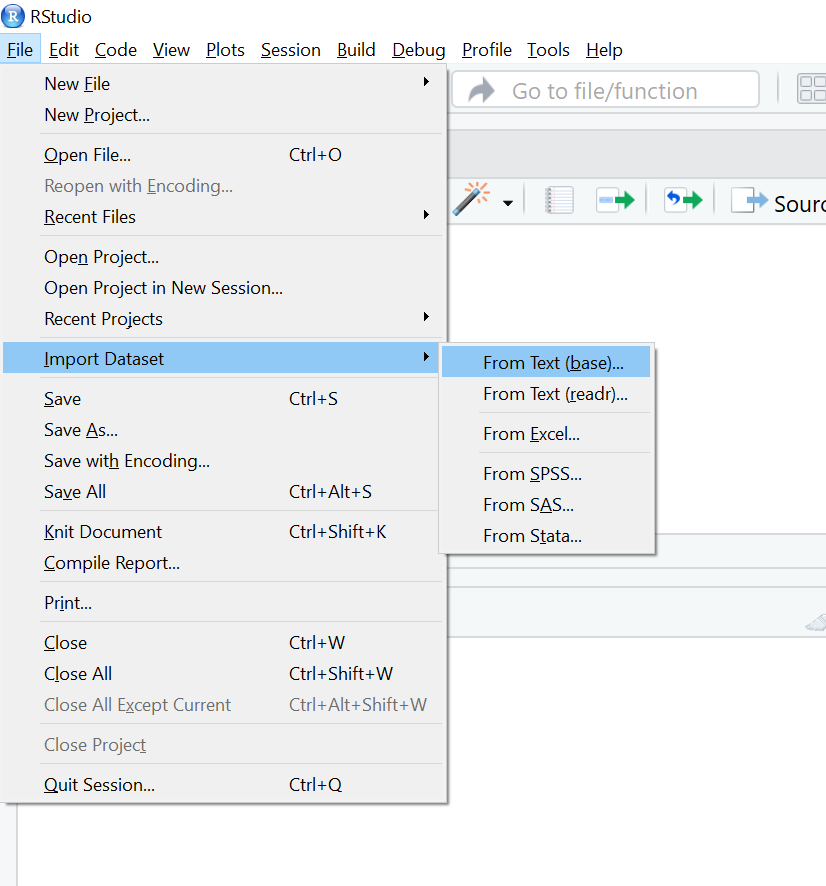
\includegraphics[scale=0.45]{img/import_data1.png}
\end{figure}

\end{frame}

\begin{frame}{Getting started}

\framesubtitle{Importing data}

\begin{figure}
\centering
  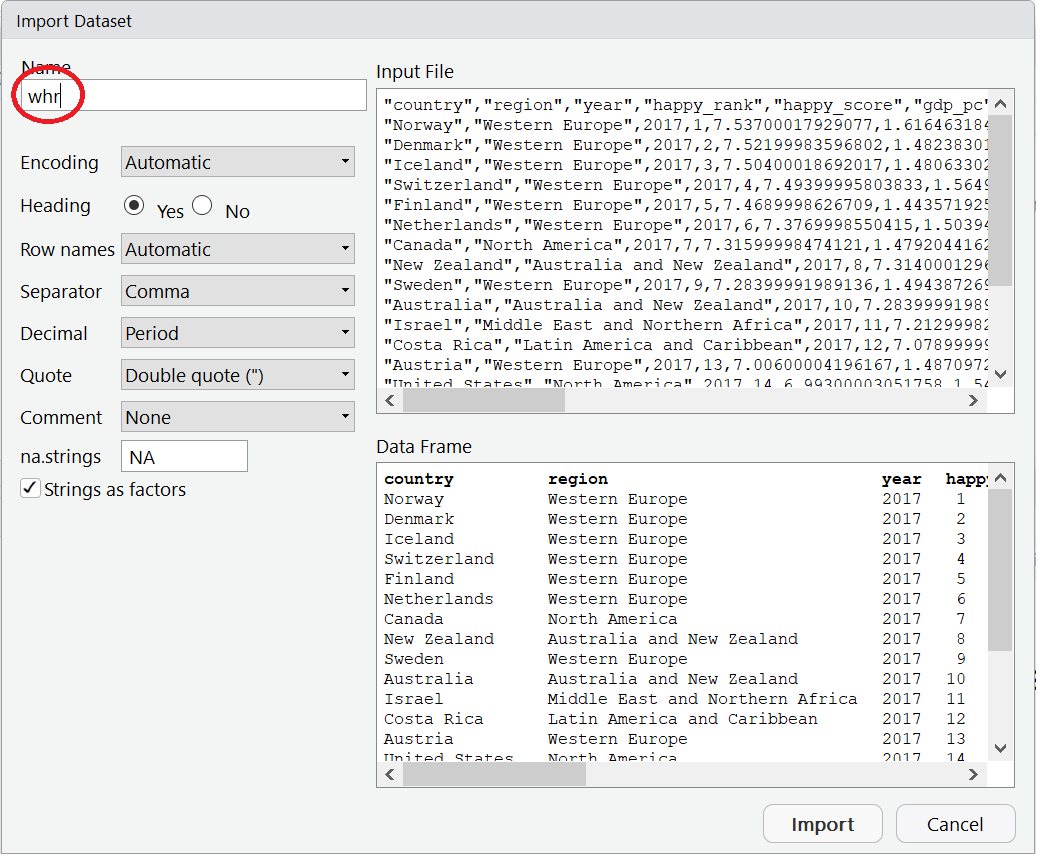
\includegraphics[scale=0.5]{img/import_data2.png}
\end{figure}

\end{frame}

\begin{frame}{RStudio interface}

\begin{figure}
\centering
  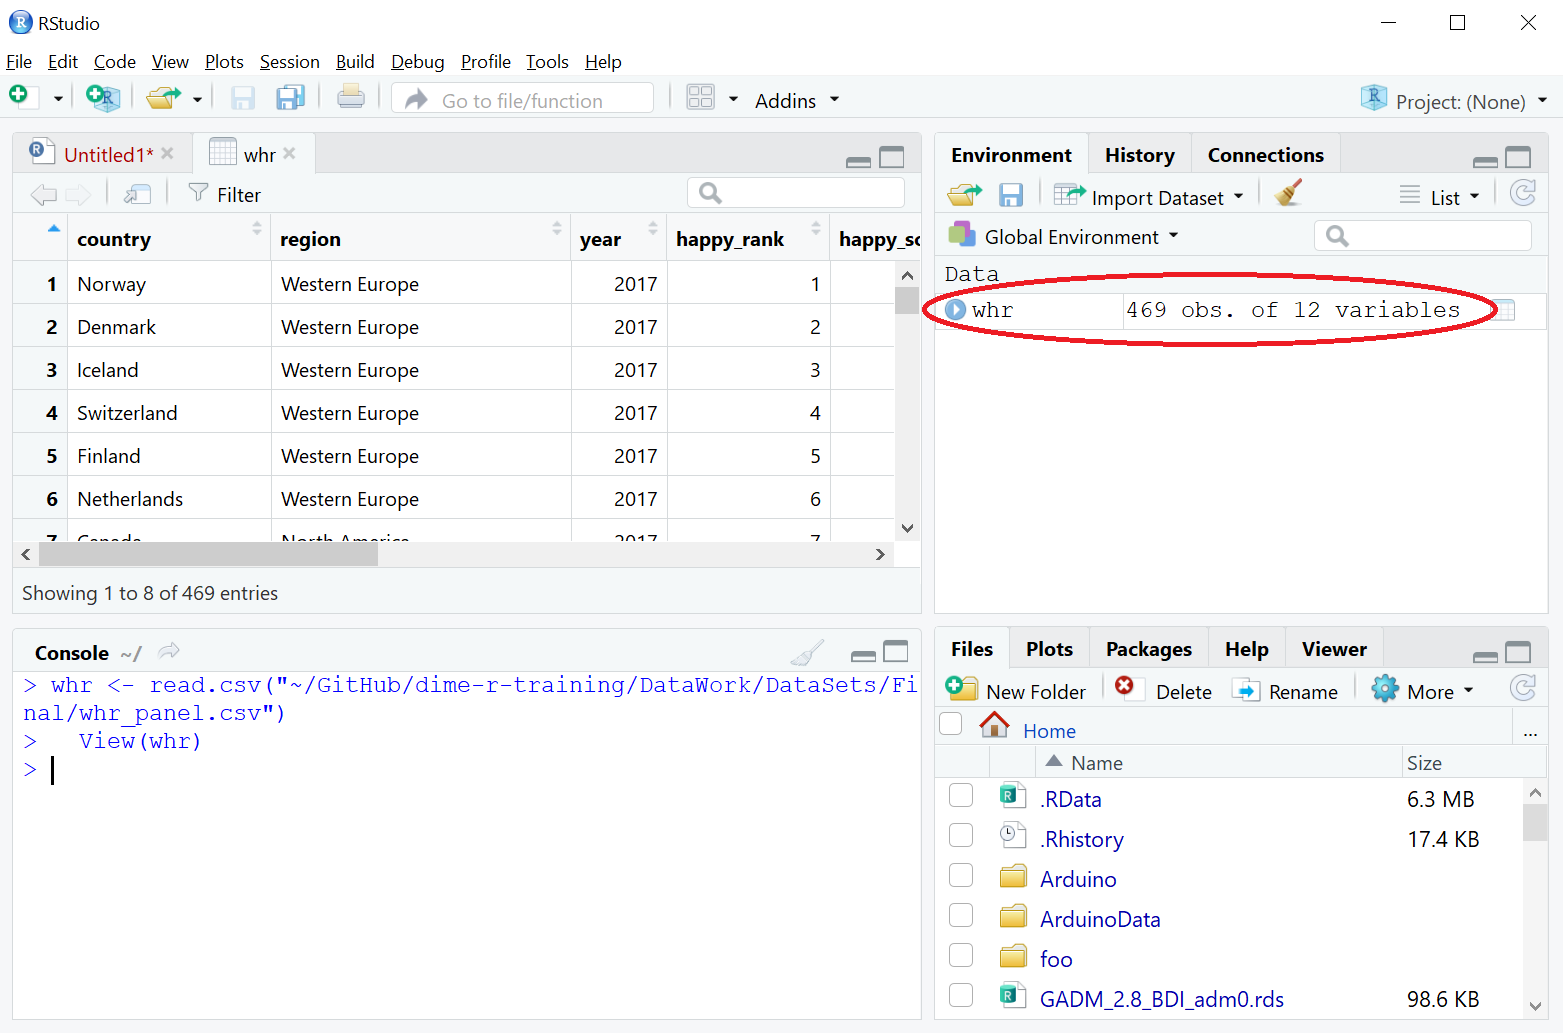
\includegraphics[width=12cm,height=7.7cm]{img/enviroment.png}
\end{figure}

\end{frame}

\begin{frame}{RStudio interface}

\begin{figure}
\centering
  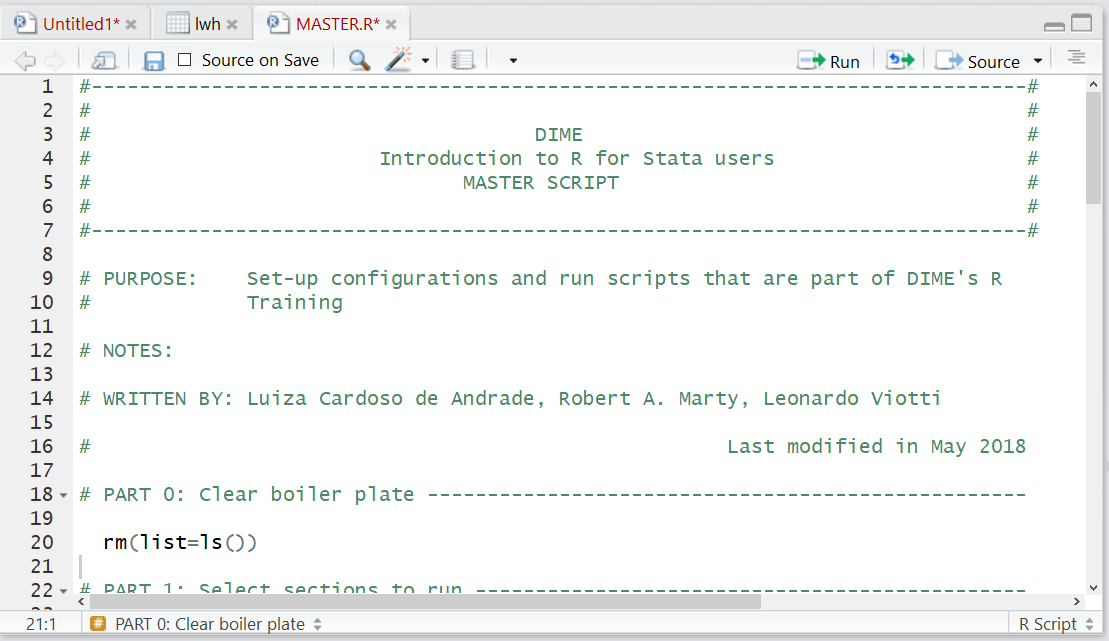
\includegraphics[width=12cm,height=7.7cm]{img/scritpt1.png}
\end{figure}

\end{frame}

\begin{frame}{RStudio interface}

\begin{figure}
\centering
  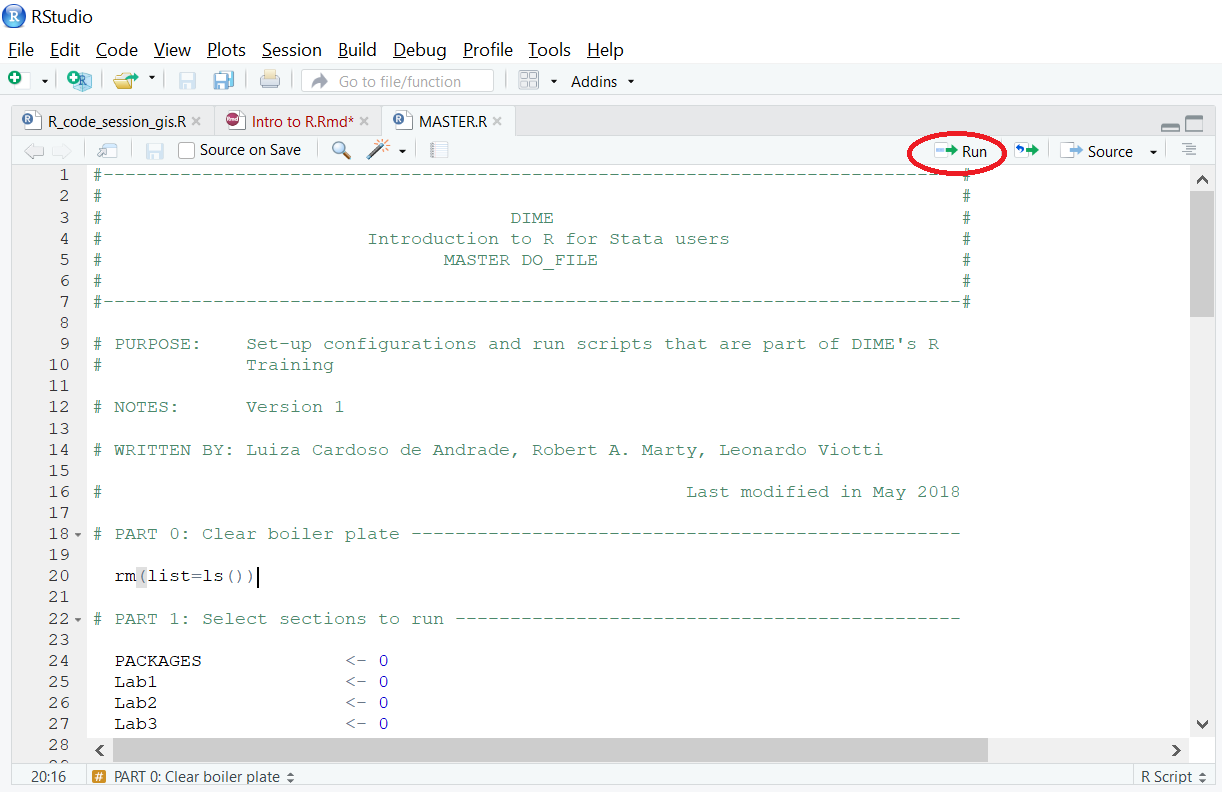
\includegraphics[width=12cm,height=7.7cm]{img/scritpt2.png}
\end{figure}

\end{frame}

\begin{frame}{RStudio interface}

\begin{figure}
\centering
  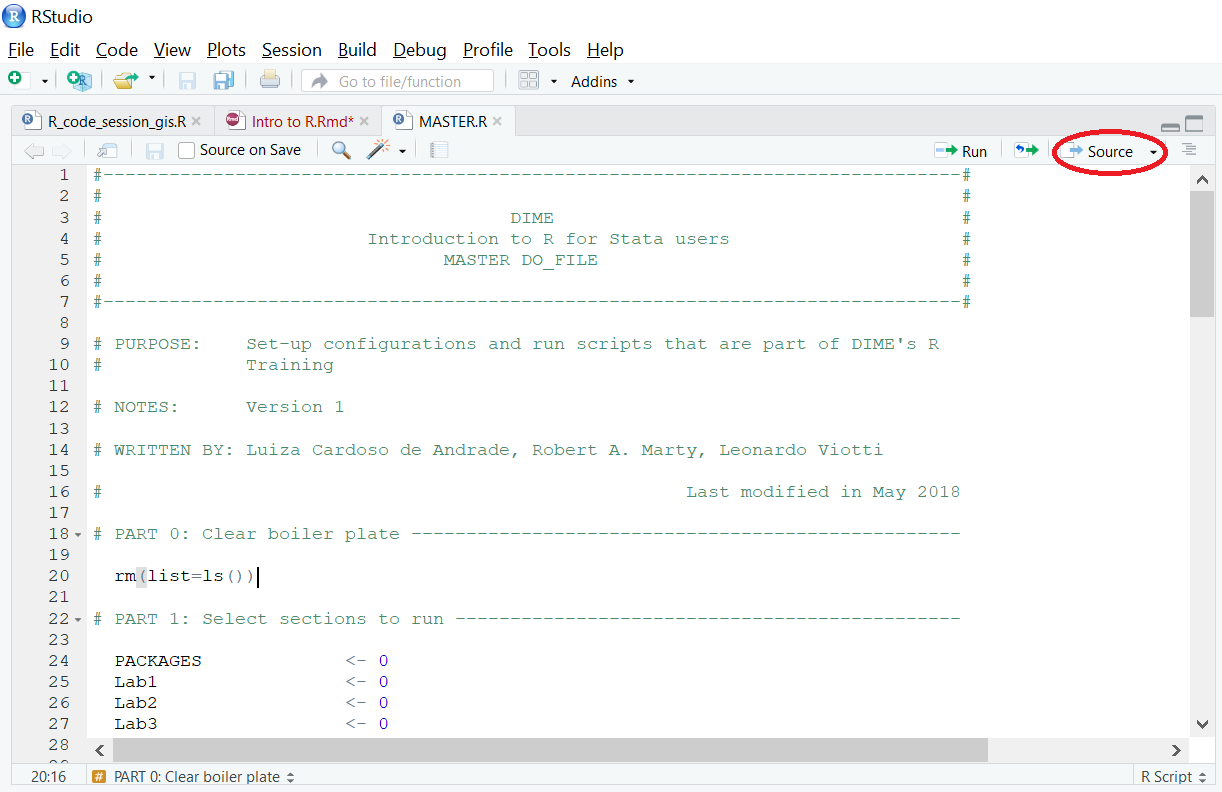
\includegraphics[width=12cm,height=7.7cm]{img/scritpt3.png}
\end{figure}

\end{frame}

\begin{frame}{RStudio interface}

\begin{figure}
\centering
  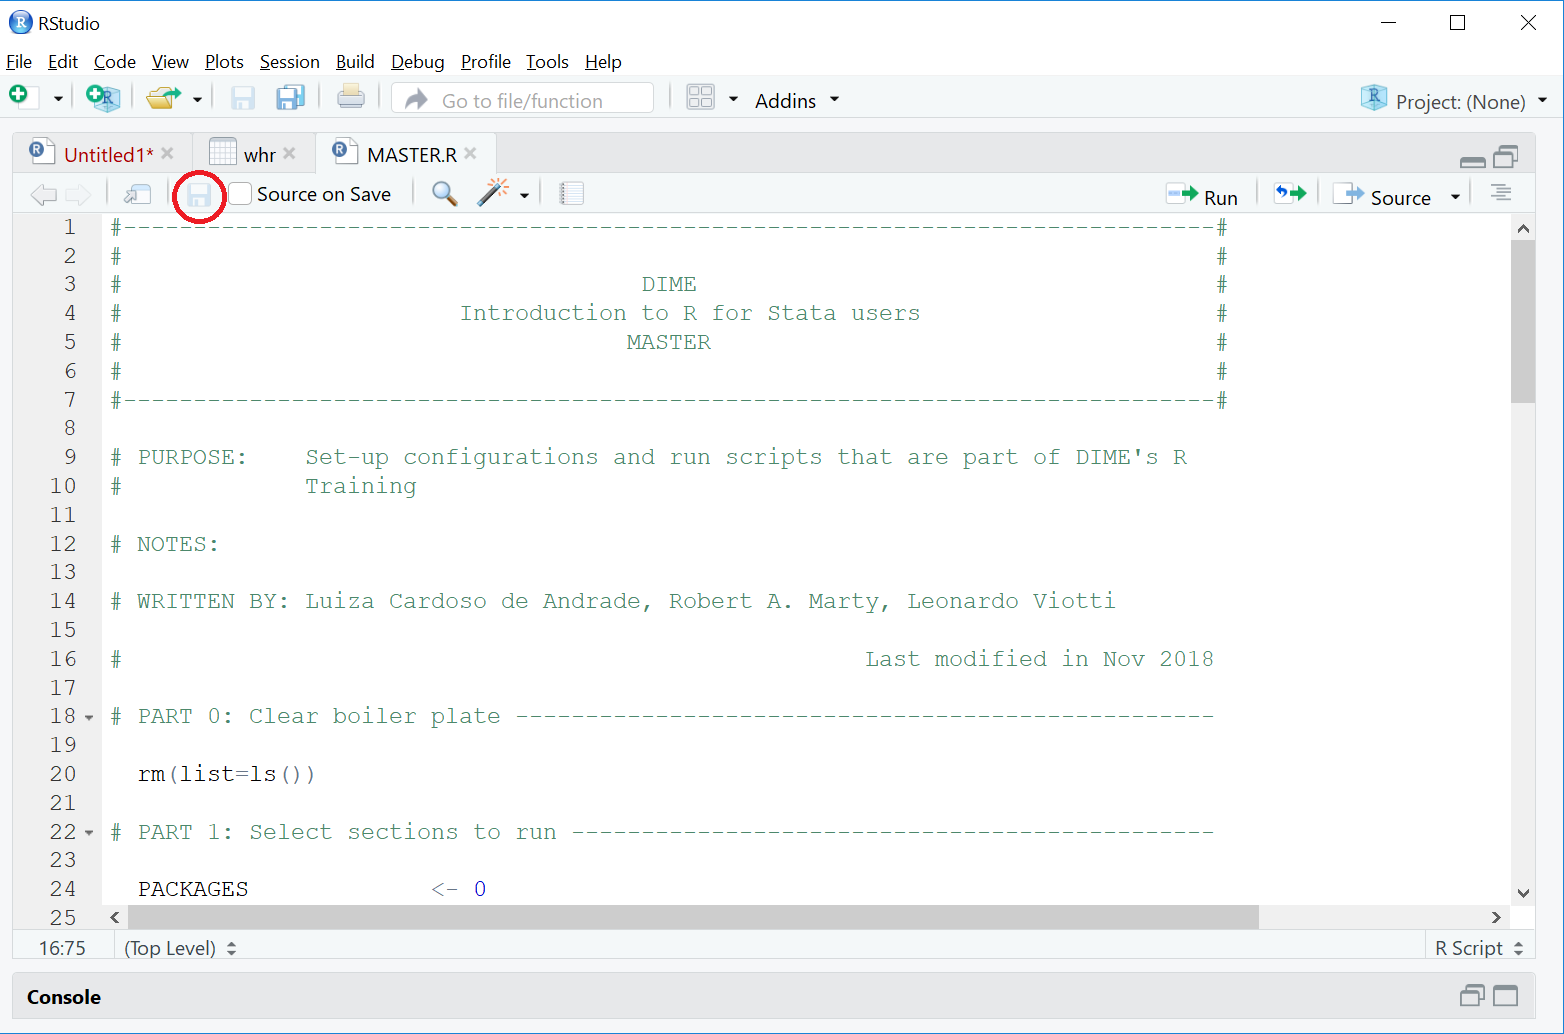
\includegraphics[width=12cm,height=7.7cm]{img/scritpt4.png}
\end{figure}

\end{frame}

\section{Data in R}\label{data-in-r}

\begin{frame}{Data in R}

\begin{itemize}
\item
  In Stata, you can open ONE dataset, and perform operations that can
  change this dataset.
\item
  You can also have other objects, such as matrices, macros and
  tempfiles, but they are secondary, and most functions only use the
  main dataset.
\item
  If you wish to do any non-permanent changes to your data, you'll need
  to preserve the original data to keep it intact.
\item
  R works in a completely different way: you can have as many datasets
  (objects) as you wish (or your computer's memory allows) and
  operations will only have lasting effects if you store them.
\end{itemize}

\end{frame}

\begin{frame}{Data in R}

\begin{itemize}
\item
  Everything that exists in R's memory -- variables, datasets, functions
  -- is an object.
\item
  An object is a chunk of data stored in the memory that has a name by
  which you call it (exactly like macros in Stata).
\item
  If you create an object, it is going to be stored in memory until you
  delete it or quit R.
\item
  Whenever you run anything you intend to use in the future, you need to
  store it as an object.
\end{itemize}

\end{frame}

\begin{frame}[fragile]{Data in R}

To better understand the idea, we're going to use the data from the
United Nations' World Happiness Report. First, let's take a look at the
data.

Type the following code to explore the data:

\begin{Shaded}
\begin{Highlighting}[]
\CommentTok{# We can use the function View() to browse the whole data}
\KeywordTok{View}\NormalTok{(whr)}

\CommentTok{# Alternatively we can print the first 6 obs. with head()}
\KeywordTok{head}\NormalTok{(whr)}
\end{Highlighting}
\end{Shaded}

\end{frame}

\begin{frame}{Data in R}

\begin{figure}
\centering
  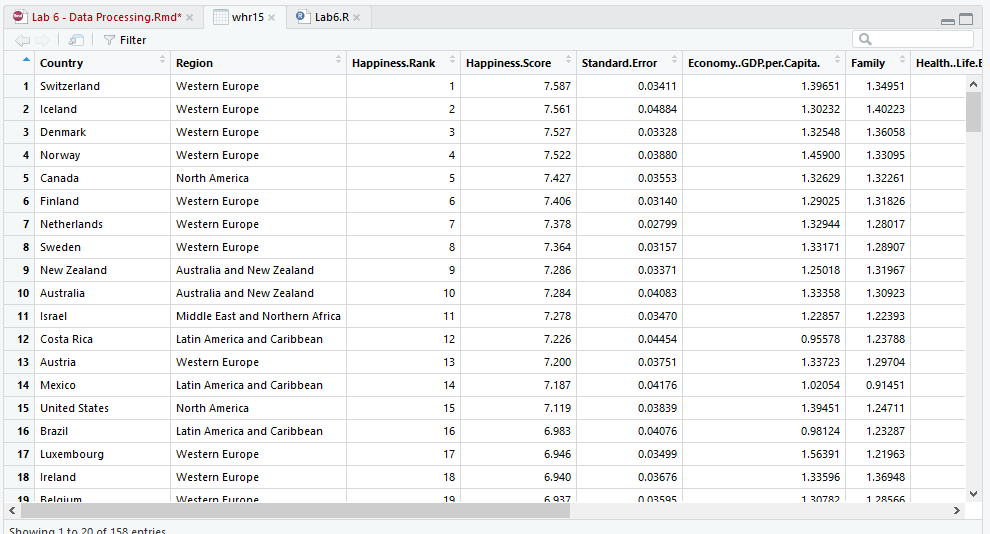
\includegraphics[scale=0.4]{img/View.png}
\end{figure}

\end{frame}

\begin{frame}[fragile]{Data in R}

\scriptsize

\begin{Shaded}
\begin{Highlighting}[]
\KeywordTok{head}\NormalTok{(whr)}
\end{Highlighting}
\end{Shaded}

\begin{verbatim}
##       country         region year happy_rank happy_score   gdp_pc   family
## 1      Norway Western Europe 2017          1       7.537 1.616463 1.533524
## 2     Denmark Western Europe 2017          2       7.522 1.482383 1.551122
## 3     Iceland Western Europe 2017          3       7.504 1.480633 1.610574
## 4 Switzerland Western Europe 2017          4       7.494 1.564980 1.516912
## 5     Finland Western Europe 2017          5       7.469 1.443572 1.540247
## 6 Netherlands Western Europe 2017          6       7.377 1.503945 1.428939
##      health   freedom trust_gov_corr generosity dystopia_res
## 1 0.7966665 0.6354226      0.3159638  0.3620122     2.277027
## 2 0.7925655 0.6260067      0.4007701  0.3552805     2.313707
## 3 0.8335521 0.6271626      0.1535266  0.4755402     2.322715
## 4 0.8581313 0.6200706      0.3670073  0.2905493     2.276716
## 5 0.8091577 0.6179509      0.3826115  0.2454828     2.430182
## 6 0.8106961 0.5853845      0.2826618  0.4704898     2.294804
\end{verbatim}

\end{frame}

\begin{frame}[fragile]{Data in R}

Now, let's try some simple manipulations. First, assume we're only
interested in data of the year 2015.

\begin{block}{Exercise 2: Subset the data}

\begin{enumerate}
\def\labelenumi{\arabic{enumi}.}
\tightlist
\item
  Subset the data set, keeping only observations where variable
  \texttt{year} equals \texttt{2015}.
\end{enumerate}

\begin{Shaded}
\begin{Highlighting}[]
\CommentTok{# To do that we'll use the subset() function}
\KeywordTok{subset}\NormalTok{(whr, year }\OperatorTok{==}\StringTok{ }\DecValTok{2015}\NormalTok{)}
\end{Highlighting}
\end{Shaded}

\begin{enumerate}
\def\labelenumi{\arabic{enumi}.}
\setcounter{enumi}{1}
\tightlist
\item
  Then, look again at the first 6 observations
\end{enumerate}

\begin{Shaded}
\begin{Highlighting}[]
\CommentTok{# Use the head() function again}
\KeywordTok{head}\NormalTok{(whr)}
\end{Highlighting}
\end{Shaded}

\end{block}

\end{frame}

\begin{frame}[fragile]{Data in R}

\scriptsize

\begin{Shaded}
\begin{Highlighting}[]
\KeywordTok{head}\NormalTok{(whr)}
\end{Highlighting}
\end{Shaded}

\begin{verbatim}
##       country         region year happy_rank happy_score   gdp_pc   family
## 1      Norway Western Europe 2017          1       7.537 1.616463 1.533524
## 2     Denmark Western Europe 2017          2       7.522 1.482383 1.551122
## 3     Iceland Western Europe 2017          3       7.504 1.480633 1.610574
## 4 Switzerland Western Europe 2017          4       7.494 1.564980 1.516912
## 5     Finland Western Europe 2017          5       7.469 1.443572 1.540247
## 6 Netherlands Western Europe 2017          6       7.377 1.503945 1.428939
##      health   freedom trust_gov_corr generosity dystopia_res
## 1 0.7966665 0.6354226      0.3159638  0.3620122     2.277027
## 2 0.7925655 0.6260067      0.4007701  0.3552805     2.313707
## 3 0.8335521 0.6271626      0.1535266  0.4755402     2.322715
## 4 0.8581313 0.6200706      0.3670073  0.2905493     2.276716
## 5 0.8091577 0.6179509      0.3826115  0.2454828     2.430182
## 6 0.8106961 0.5853845      0.2826618  0.4704898     2.294804
\end{verbatim}

\end{frame}

\begin{frame}[fragile]{Data in R}

We can see that nothing happened to the original data. This happens
because we didn't store the edit we made anywhere.

\begin{block}{To store an object, we use the assignment operator
(\texttt{\textless{}-}):}

\begin{Shaded}
\begin{Highlighting}[]
\CommentTok{# Assign the Answer to the Ultimate Question of Life, }
\CommentTok{# the Universe, and Everything}
\NormalTok{x <-}\StringTok{ }\DecValTok{42}
\end{Highlighting}
\end{Shaded}

From now on, \emph{x} is associated with the stored value (until you
replace it delete it or close R).

\end{block}

\end{frame}

\begin{frame}[fragile]{Data in R}

\begin{block}{Exercise 3: Create an object}

Create a new data set, called \texttt{whr2015}, that is a subset of the
\texttt{whr} data set containing only data from the year 2015.

\begin{Shaded}
\begin{Highlighting}[]
\CommentTok{# Using the same function but now assigning it to an object}
\NormalTok{whr2015 <-}\StringTok{ }\KeywordTok{subset}\NormalTok{(whr, year }\OperatorTok{==}\StringTok{ }\DecValTok{2015}\NormalTok{)}

\CommentTok{# Display the 5 first obs. of the new data}
\KeywordTok{head}\NormalTok{(whr2015)}

\CommentTok{# Notice that we still have the original data set intact}
\KeywordTok{head}\NormalTok{(whr)}
\end{Highlighting}
\end{Shaded}

\end{block}

\end{frame}

\begin{frame}[fragile]{Data in R}

\scriptsize

\begin{Shaded}
\begin{Highlighting}[]
\KeywordTok{head}\NormalTok{(whr2015)}
\end{Highlighting}
\end{Shaded}

\begin{verbatim}
##         country         region year happy_rank happy_score  gdp_pc  family
## 313 Switzerland Western Europe 2015          1       7.587 1.39651 1.34951
## 314     Iceland Western Europe 2015          2       7.561 1.30232 1.40223
## 315     Denmark Western Europe 2015          3       7.527 1.32548 1.36058
## 316      Norway Western Europe 2015          4       7.522 1.45900 1.33095
## 317      Canada  North America 2015          5       7.427 1.32629 1.32261
## 318     Finland Western Europe 2015          6       7.406 1.29025 1.31826
##      health freedom trust_gov_corr generosity dystopia_res
## 313 0.94143 0.66557        0.41978    0.29678      2.51738
## 314 0.94784 0.62877        0.14145    0.43630      2.70201
## 315 0.87464 0.64938        0.48357    0.34139      2.49204
## 316 0.88521 0.66973        0.36503    0.34699      2.46531
## 317 0.90563 0.63297        0.32957    0.45811      2.45176
## 318 0.88911 0.64169        0.41372    0.23351      2.61955
\end{verbatim}

\end{frame}

\begin{frame}[fragile]{Data in R}

\scriptsize

\begin{Shaded}
\begin{Highlighting}[]
\KeywordTok{head}\NormalTok{(whr)}
\end{Highlighting}
\end{Shaded}

\begin{verbatim}
##       country         region year happy_rank happy_score   gdp_pc   family
## 1      Norway Western Europe 2017          1       7.537 1.616463 1.533524
## 2     Denmark Western Europe 2017          2       7.522 1.482383 1.551122
## 3     Iceland Western Europe 2017          3       7.504 1.480633 1.610574
## 4 Switzerland Western Europe 2017          4       7.494 1.564980 1.516912
## 5     Finland Western Europe 2017          5       7.469 1.443572 1.540247
## 6 Netherlands Western Europe 2017          6       7.377 1.503945 1.428939
##      health   freedom trust_gov_corr generosity dystopia_res
## 1 0.7966665 0.6354226      0.3159638  0.3620122     2.277027
## 2 0.7925655 0.6260067      0.4007701  0.3552805     2.313707
## 3 0.8335521 0.6271626      0.1535266  0.4755402     2.322715
## 4 0.8581313 0.6200706      0.3670073  0.2905493     2.276716
## 5 0.8091577 0.6179509      0.3826115  0.2454828     2.430182
## 6 0.8106961 0.5853845      0.2826618  0.4704898     2.294804
\end{verbatim}

\end{frame}

\begin{frame}{Data in R}

You can also see that your environment pane now has two objects:

\begin{figure}
\centering
  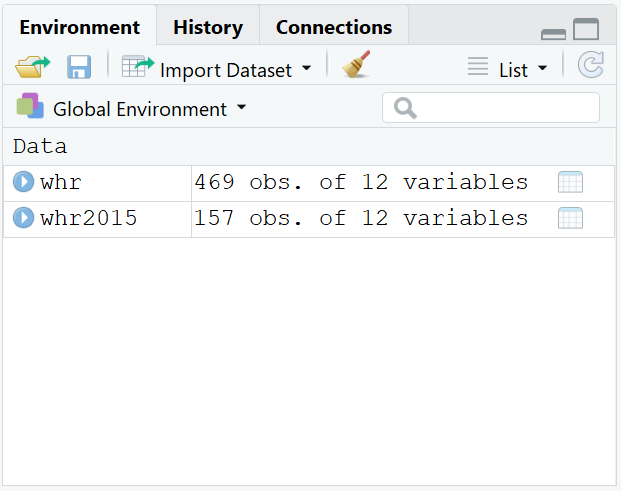
\includegraphics[scale=0.5]{img/enviroment_2vars.png}
\end{figure}

\end{frame}

\begin{frame}{Data in R}

\begin{block}{Two important concepts to take note:}

\begin{enumerate}
\def\labelenumi{\arabic{enumi}.}
\tightlist
\item
  In R, if you want to change your data, you need to store it in an
  object.
\item
  It is possible to simply replace the original data. This happens if
  you assign the new object to the same name as the original.
\item
  Print (display) is built into R. If you execute any action without
  storing it, R will simply print the results of that action but won't
  save anything in the memory.
\end{enumerate}

\end{block}

\end{frame}

\section{R objects}\label{r-objects}

\begin{frame}{R objects}

Objects are the building blocks of R programming. T his section will
explore some of the most common.

This will give you the foundation to explore your data and construct
analytical outputs.

\end{frame}

\begin{frame}{R objects}

Here are the types of object we will cover today:

\begin{itemize}
\tightlist
\item
  \textbf{Vectors:} an uni-dimensional object that stores a sequence of
  values
\item
  \textbf{Data frames:} a combination of different vectors of the same
  length (the same as your data set in Stata)
\item
  \textbf{Lists:} a multidimensional object that can store several
  objects of different dimension
\end{itemize}

\end{frame}

\begin{frame}[fragile]{R objects}

\framesubtitle{Vectors}

A vector is an uni-dimensional object composed by one or more scalars of
the same type.

\begin{block}{Use the following code to create vectors in two different
ways}

\begin{Shaded}
\begin{Highlighting}[]
\CommentTok{# Creating a vector with the c() function}
\NormalTok{v1 <-}\StringTok{ }\KeywordTok{c}\NormalTok{(}\DecValTok{1}\NormalTok{,}\DecValTok{1}\NormalTok{,}\DecValTok{2}\NormalTok{,}\DecValTok{3}\NormalTok{,}\DecValTok{5}\NormalTok{)}

\CommentTok{# Alternative way to create an evenly spaced vector}
\NormalTok{v2 <-}\StringTok{ }\DecValTok{1}\OperatorTok{:}\DecValTok{5}
\end{Highlighting}
\end{Shaded}

\end{block}

\begin{block}{You can use brackets for indexing}

\begin{Shaded}
\begin{Highlighting}[]
\CommentTok{# Print the 4th element of the vector}
\NormalTok{v2[}\DecValTok{4}\NormalTok{]}
\end{Highlighting}
\end{Shaded}

\begin{verbatim}
## [1] 4
\end{verbatim}

\end{block}

\end{frame}

\begin{frame}[fragile]{R objects}

\framesubtitle{Vectors}

To R, each of the columns of \texttt{whr} is a vector.

\begin{block}{Calling a vector from a \texttt{data.frame} column}

We use the \texttt{\$} to call vectors (variables) by their names in a
\texttt{data.frame}

\end{block}

\begin{block}{Type the following code:}

\begin{Shaded}
\begin{Highlighting}[]
\CommentTok{# Create a vector with the values of the `year` variable}
\NormalTok{year_vec <-}\StringTok{ }\NormalTok{whr}\OperatorTok{$}\NormalTok{year}

\CommentTok{# See the 3 first elements of the year column}
\NormalTok{whr}\OperatorTok{$}\NormalTok{year[}\DecValTok{1}\OperatorTok{:}\DecValTok{3}\NormalTok{]}
\end{Highlighting}
\end{Shaded}

\begin{verbatim}
## [1] 2017 2017 2017
\end{verbatim}

\end{block}

\end{frame}

\begin{frame}[fragile]{R objects}

\framesubtitle{Data Frames}

The \texttt{whr} and \texttt{whr2015} objects are both data frames. You
can also construct a new data frame from scratch by combining vectors
with the same number of elements .

\begin{block}{Now, type the following code to create a new data frame}

\begin{Shaded}
\begin{Highlighting}[]
\CommentTok{# Dataframe created by biding vectors}
\NormalTok{df1 <-}\StringTok{ }\KeywordTok{data.frame}\NormalTok{(v1,v2)}
\NormalTok{df1}
\end{Highlighting}
\end{Shaded}

\begin{verbatim}
##   v1 v2
## 1  1  1
## 2  1  2
## 3  2  3
## 4  3  4
## 5  5  5
\end{verbatim}

\end{block}

\end{frame}

\begin{frame}[fragile]{R objects}

\framesubtitle{Data Frames}

Since a data frame has two dimensions, you can use indexing on both:

\begin{block}{Numeric indexing}

\begin{Shaded}
\begin{Highlighting}[]
\CommentTok{# The first column of whr}
\NormalTok{whr[,}\DecValTok{1}\NormalTok{]}

\CommentTok{# The 45th line of whr}
\NormalTok{whr[}\DecValTok{45}\NormalTok{,]}

\CommentTok{# Or the 45th element of the first line}
\NormalTok{whr[}\DecValTok{45}\NormalTok{,}\DecValTok{1}\NormalTok{]}
\end{Highlighting}
\end{Shaded}

\end{block}

\end{frame}

\begin{frame}[fragile]{R objects}

\framesubtitle{Data Frames}

Alternatively, you can use the column names for indexing, which is the
same as using the \texttt{\$} sign.

\begin{block}{Names indexing}

\begin{Shaded}
\begin{Highlighting}[]
\CommentTok{# Or the 22th element of the country column}
\NormalTok{whr[}\DecValTok{22}\NormalTok{,}\StringTok{"country"}\NormalTok{] }\CommentTok{# The same as whr$country[22]}
\end{Highlighting}
\end{Shaded}

\begin{verbatim}
## [1] Brazil
## 164 Levels: Afghanistan Albania Algeria Angola Argentina ... Zimbabwe
\end{verbatim}

\end{block}

\end{frame}

\begin{frame}[fragile]{R objects}

\framesubtitle{Data Frames}

Lists are more complex objects that can contain many objects of
different classes and dimensions.

Lists are fancy and can have a lot of functionalities and attributes.
They are the output of many functions and are used to construct complex
objects.

It would be beyond the scope of this introduction to go deep into them,
but here's a quick example

\begin{block}{Combine several objects of different types in a list}

\begin{Shaded}
\begin{Highlighting}[]
\CommentTok{# Use the list() function}
\NormalTok{lst <-}\StringTok{ }\KeywordTok{list}\NormalTok{(v1, df1, }\DecValTok{45}\NormalTok{)}
\end{Highlighting}
\end{Shaded}

Print the list yourself to see how it looks like.

\end{block}

\end{frame}

\begin{frame}[fragile]{R objects}

\framesubtitle{Lists}

\scriptsize

\begin{Shaded}
\begin{Highlighting}[]
\CommentTok{# Check the contents of lst}
\KeywordTok{print}\NormalTok{(lst)}
\end{Highlighting}
\end{Shaded}

\begin{verbatim}
## [[1]]
## [1] 1 1 2 3 5
## 
## [[2]]
##   v1 v2
## 1  1  1
## 2  1  2
## 3  2  3
## 4  3  4
## 5  5  5
## 
## [[3]]
## [1] 45
\end{verbatim}

\end{frame}

\section{Basic types of data}\label{basic-types-of-data}

\begin{frame}{Basic types of data}

R has different kinds of data that can be recorded inside objects. They
are very similar to what you have in Stata, and the main types are
string, integer, numeric, factor and boolean.

Let's start with the simpler ones:

\begin{block}{Strings}

A sequence of characters and are usually represented between double
quotes. They can contain single letters, words, phrases or even some
longer text.

\end{block}

\begin{block}{Integer and numeric}

As in Stata, these are two different ways to store numbers. They are
different because they use memory differently. As default, R stores
numbers in the numeric format (double).

\end{block}

\end{frame}

\begin{frame}[fragile]{Basic types of data}

\framesubtitle{Strings}

Now we'll use string data to practice some basic object manipulations in
R.

\begin{block}{Exercise 4: Create a vector of strings}

Create two string vector containing the names of commonly used
statistical software in order of importance:

\begin{Shaded}
\begin{Highlighting}[]
\CommentTok{# Creating string vector}
\NormalTok{str_vec <-}\StringTok{ }\KeywordTok{c}\NormalTok{(}\StringTok{"R"}\NormalTok{,}
             \StringTok{"Python"}\NormalTok{,}
             \StringTok{"SAS"}\NormalTok{,}
             \StringTok{"Excel"}\NormalTok{,}
             \StringTok{"Stata"}\NormalTok{)}
\end{Highlighting}
\end{Shaded}

Now print them to check them out.

\end{block}

\end{frame}

\begin{frame}[fragile]{Basic types of data}

\framesubtitle{Strings}

\begin{block}{Exercise 5: Concatenate strings}

\begin{enumerate}
\def\labelenumi{\arabic{enumi}.}
\tightlist
\item
  Create a scalar (a vector of one element) containing the phrase ``is
  better than'' and cal it \texttt{str\_scalar}.
\item
  Use the function \texttt{paste()} with 3 arguments separated by
  commas:
\end{enumerate}

\begin{itemize}
\tightlist
\item
  The first argument as the 1st element of \texttt{str\_vec}.
\item
  The second argument as the \texttt{str\_scalar}.
\item
  The third argument as the 5th element of \texttt{str\_vec}.
\end{itemize}

\begin{enumerate}
\def\labelenumi{\arabic{enumi}.}
\setcounter{enumi}{2}
\tightlist
\item
  If you're not sure where to start, type:
\end{enumerate}

\begin{Shaded}
\begin{Highlighting}[]
\KeywordTok{help}\NormalTok{(paste)}
\end{Highlighting}
\end{Shaded}

\end{block}

\end{frame}

\begin{frame}[fragile]{Basic types of data}

\framesubtitle{Strings}

\begin{Shaded}
\begin{Highlighting}[]
\NormalTok{### Using the paste function to combine strings}

\CommentTok{# Scalar}
\NormalTok{str_scalar <-}\StringTok{ "is better than"}

\CommentTok{# Using the paste() function}
\KeywordTok{paste}\NormalTok{(str_vec[}\DecValTok{1}\NormalTok{], str_scalar, str_vec[}\DecValTok{5}\NormalTok{])}
\end{Highlighting}
\end{Shaded}

\begin{verbatim}
## [1] "R is better than Stata"
\end{verbatim}

\end{frame}

\section{First R code}\label{first-r-code}

\begin{frame}{First R code}

\framesubtitle{Coding workflow}

\begin{enumerate}
\def\labelenumi{\arabic{enumi}.}
\tightlist
\item
  Pick problem
\item
  Think of how to solve the problem
\item
  Write code little by little:

  \begin{itemize}
  \tightlist
  \item
    Experiment with the instructions you think will work
  \item
    Write the ones that do work in your code
  \item
    Run all your code at once to see if it works\\
  \item
    Repeat!
  \end{itemize}
\item
  Export your results.
\end{enumerate}

\end{frame}

\begin{frame}{First R code}

\framesubtitle{Coding workflow}

\begin{block}{TIP:}

There are two different ways use code:

\begin{enumerate}
\def\labelenumi{\arabic{enumi}.}
\item
  Give instructions for the computer to give you some information, these
  we usually type directly in the console.
\item
  The instructions for the computer to perform the actual tasks need for
  your analysis. These are the ones you want in your script.
\end{enumerate}

\end{block}

\end{frame}

\begin{frame}{First R code}

\begin{block}{Exercise 6}

Write code to produce a line graph containing the happiness index over
the years for Rwanda and it's neighbors.

\end{block}

\end{frame}

\begin{frame}{First R code}

\includegraphics{Lab_0_-_Intro_to_R_files/figure-beamer/unnamed-chunk-26-1.pdf}

\end{frame}

\begin{frame}[fragile]{First R code}

\begin{block}{Exercise 6 - Instructions}

\begin{enumerate}
\def\labelenumi{\arabic{enumi}.}
\tightlist
\item
  Clean your memmory by typing \texttt{rm(list\ =\ rm())} and pressing
  enter.
\item
  Open template script called Lab 0 - First R code.R
\item
  Follow the instructions in the script.
\end{enumerate}

\end{block}

\end{frame}

\begin{frame}{First R code}

\begin{block}{Exercise 6 - Update your data!}

\begin{enumerate}
\def\labelenumi{\arabic{enumi}.}
\tightlist
\item
  Now, chage the data by replacing the name of the file in the code with
  whr\_panel\_18.csv
\item
  Re run your code without changing anything else.
\end{enumerate}

\end{block}

\end{frame}

\section{Help, Google and
Stackoverflow}\label{help-google-and-stackoverflow}

\begin{frame}[fragile]{Help, Google and Stackoverflow}

Help in R works very much like in Stata: the help files usually start
with a brief description of the function, explain its syntax and
arguments and list a few examples. There are two ways to access help
files:

\begin{block}{Exercise 7: Use help}

\begin{Shaded}
\begin{Highlighting}[]
\CommentTok{# The help() function}
\KeywordTok{help}\NormalTok{(summary)}

\CommentTok{# and its abbreviation}
\NormalTok{?summary}
\end{Highlighting}
\end{Shaded}

\end{block}

\end{frame}

\begin{frame}{Help, Google and Stackoverflow}

\begin{itemize}
\item
  The biggest difference, however, is that R has a much wider user
  community and it has a lot more online resources.
\item
  For instance, in 2014, Stata had 11 dedicated blogs written by users,
  while R had 550.\footnote<.->{Check
    \url{http://r4stats.com/articles/popularity/} for more.}
\item
  The most powerful problem-solving tool in R, however, is Google.
  Searching the something yields tons of results.
\item
  Often that means a Stack Overflow page where someone asked the same
  question and several people gave different answers. Here's a typical
  example:
  \url{https://stackoverflow.com/questions/1660124/how-to-sum-a-variable-by-group}
\end{itemize}

\end{frame}

\section{Useful resources}\label{useful-resources}

\begin{frame}{Useful resources}

\textcolor{myColor}{Blogs and online courses:}

\begin{itemize}
\item
  Surviving graduate econometrics with R:
  \url{https://thetarzan.wordpress.com/2011/05/24/surviving-graduate-econometrics-with-r-the-basics-1-of-8/}
\item
  An Introduction to R at \url{https://cran.r-project.org/}
\item
  R programming in Coursera:
  \url{https://www.coursera.org/learn/r-programming}
\item
  Try R in Code School: \url{http://tryr.codeschool.com/}
\item
  R programming for dummies: \url{http://www.dummies.com/programming/r/}
\item
  R bloggers: \url{https://www.r-bloggers.com/}
\item
  R statistics blog: \url{https://www.r-statistics.com/}
\item
  The R graph gallery: \url{https://www.r-graph-gallery.com/}
\end{itemize}

\end{frame}

\begin{frame}{Useful resources}

\textcolor{myColor}{Books:}

\begin{itemize}
\item
  R for Stata Users - Robert A. Muenchen and Joseph Hilbe
\item
  R Graphics Cookbook - Winston Chang
\item
  R for Data Science - Hadley Wickha and Garrett Grolemund
\end{itemize}

\end{frame}

\begin{frame}

\huge Thank you!

\end{frame}

\section{Appendix}\label{appendix}

\begin{frame}[fragile]{Appendix - Syntax}

R's syntax is a bit heavier than Stata's:

\begin{itemize}
\tightlist
\item
  Parentheses to separate function names from its arguments.
\item
  Commas to separate arguments.
\item
  For comments we use the \texttt{\#} sign.
\item
  You can have line breaks inside function statements.
\item
  In R, functions can be treated much like any other object Therefore,
  they can be passed as arguments to other functions.
\end{itemize}

Similarly to Stata:

\begin{itemize}
\tightlist
\item
  Square brackets are used for indexing.
\item
  Curly braces are used for loops and if statements.
\item
  Largely ignores white spaces.
\end{itemize}

\end{frame}

\begin{frame}{Appendix - RStudio interface}

\begin{block}{Script}

Where you write your code. Just like a do file.

\end{block}

\begin{block}{Console}

Where your results and messages will be displayed. But you can also type
commands directly into the console, as in Stata.

\end{block}

\begin{block}{Environment}

What's in R's memory.

\end{block}

\begin{block}{The 4th pane}

Can display different things, including plots you create, packages
loaded and help files.

\end{block}

\end{frame}

\begin{frame}[fragile]{Appendix - Matrices}

A matrix a bi-dimensional object composed by one or more vectors of the
same type.

\begin{block}{Type the following code to test two different ways of
creating matrices}

\begin{Shaded}
\begin{Highlighting}[]
\CommentTok{# Matrix created by joining two vectors:}
\NormalTok{m1 <-}\StringTok{ }\KeywordTok{cbind}\NormalTok{(v1,v1)}

\CommentTok{# Matrix using the }
\NormalTok{m2 <-}\StringTok{ }\KeywordTok{matrix}\NormalTok{(}\KeywordTok{c}\NormalTok{(}\DecValTok{1}\NormalTok{,}\DecValTok{1}\NormalTok{,}\DecValTok{2}\NormalTok{,}\DecValTok{3}\NormalTok{,}\DecValTok{5}\NormalTok{,}\DecValTok{8}\NormalTok{), }\DataTypeTok{ncol =} \DecValTok{2}\NormalTok{)}
\end{Highlighting}
\end{Shaded}

\end{block}

\end{frame}

\begin{frame}[fragile]{Appendix - Matrices}

\begin{block}{Now use the following code to check the elements of these
matrices by indexing}

\begin{Shaded}
\begin{Highlighting}[]
\CommentTok{# Matrix indexing: typing matrix[i,j] will give you}
\CommentTok{# the element in the ith row and jth column of that matrix}
\CommentTok{#m2[1,2]}

\CommentTok{# Matrix indexing: typing matrix[i,] will give you the}
\CommentTok{# ith row of that matrix}
\NormalTok{m1[}\DecValTok{1}\NormalTok{,]}

\CommentTok{# Matrix indexing: typing matrix[,j] will give you the}
\CommentTok{# jth column of that matrix (as a vector)}
\NormalTok{m1[,}\DecValTok{2}\NormalTok{]}
\end{Highlighting}
\end{Shaded}

\end{block}

\end{frame}

\begin{frame}[fragile]{Appendix - Advanced types of data - Factors}

\framesubtitle{Factors}

\begin{block}{Create a factor verctor using the following code}

\begin{Shaded}
\begin{Highlighting}[]
\CommentTok{# Basic factor vector}
\NormalTok{num_vec <-}\StringTok{ }\KeywordTok{c}\NormalTok{(}\DecValTok{1}\NormalTok{,}\DecValTok{2}\NormalTok{,}\DecValTok{2}\NormalTok{,}\DecValTok{3}\NormalTok{,}\DecValTok{1}\NormalTok{,}\DecValTok{2}\NormalTok{,}\DecValTok{3}\NormalTok{,}\DecValTok{3}\NormalTok{,}\DecValTok{1}\NormalTok{,}\DecValTok{2}\NormalTok{,}\DecValTok{3}\NormalTok{,}\DecValTok{3}\NormalTok{,}\DecValTok{1}\NormalTok{)}
\NormalTok{fac_vec <-}\StringTok{ }\KeywordTok{factor}\NormalTok{(num_vec)}

\CommentTok{# A bit fancier factor vector}
\NormalTok{fac_vec <-}\StringTok{ }\KeywordTok{factor}\NormalTok{(num_vec,}\DataTypeTok{labels=}\KeywordTok{c}\NormalTok{(}\StringTok{"A"}\NormalTok{,}\StringTok{"B"}\NormalTok{,}\StringTok{"C"}\NormalTok{))}

\CommentTok{# Change labels}
\KeywordTok{levels}\NormalTok{(fac_vec) =}\StringTok{ }\KeywordTok{c}\NormalTok{(}\StringTok{'One'}\NormalTok{,}\StringTok{'Two'}\NormalTok{,}\StringTok{'Three'}\NormalTok{)}
\end{Highlighting}
\end{Shaded}

\end{block}

\end{frame}

\begin{frame}[fragile]{Appendix - Numbers and integers}

\begin{block}{Two scalars, one with a round number the other with a
fractional part}

\begin{Shaded}
\begin{Highlighting}[]
\CommentTok{# a numeric scalar with an integer number}
\NormalTok{int <-}\StringTok{ }\DecValTok{13}
\NormalTok{num <-}\StringTok{ }\FloatTok{12.99}
\end{Highlighting}
\end{Shaded}

\end{block}

\end{frame}

\begin{frame}[fragile]{Appendix - Numbers and integers}

\begin{block}{Now we can see the objects classes with the \emph{class()}
function and test it with the \emph{is.integer()} and
\emph{is.numeric()} functions.}

\begin{Shaded}
\begin{Highlighting}[]
\CommentTok{# you can see the number's format using the class function:}
\KeywordTok{class}\NormalTok{(int)}
\end{Highlighting}
\end{Shaded}

\begin{verbatim}
## [1] "numeric"
\end{verbatim}

\begin{Shaded}
\begin{Highlighting}[]
\KeywordTok{class}\NormalTok{(num)}
\end{Highlighting}
\end{Shaded}

\begin{verbatim}
## [1] "numeric"
\end{verbatim}

\begin{Shaded}
\begin{Highlighting}[]
\CommentTok{# you can test the class with the is. method}
\KeywordTok{is.integer}\NormalTok{(int)}
\end{Highlighting}
\end{Shaded}

\begin{verbatim}
## [1] FALSE
\end{verbatim}

\begin{Shaded}
\begin{Highlighting}[]
\KeywordTok{is.numeric}\NormalTok{(int)}
\end{Highlighting}
\end{Shaded}

\begin{verbatim}
## [1] TRUE
\end{verbatim}

Did you notice anything strange? That happens because the default way R
stores numbers is \emph{numeric}, which is equivalent to \emph{double}
in Stata.

\end{block}

\end{frame}

\begin{frame}[fragile]{Appendix - Numbers and integers}

\framesubtitle{Numbers and integers}

We can, however, coerce objects into different classes. We just need to
be careful because the result might not be what we're expecting.

\begin{block}{Use the \emph{as.integer()} and \emph{round()} functions
on the \emph{num} object to see the difference:}

\begin{Shaded}
\begin{Highlighting}[]
\KeywordTok{as.integer}\NormalTok{(num)}
\end{Highlighting}
\end{Shaded}

\begin{verbatim}
## [1] 12
\end{verbatim}

\begin{Shaded}
\begin{Highlighting}[]
\CommentTok{# and}

\KeywordTok{round}\NormalTok{(num)}
\end{Highlighting}
\end{Shaded}

\begin{verbatim}
## [1] 13
\end{verbatim}

Advanced types of data

\end{block}

\end{frame}

\begin{frame}[fragile]{Advanced types of data}

R also has other more complex ways of storing data. These are the most
used:

\begin{block}{Factors}

Factors are numeric categorical values with text label, equivalent to
labelled variables in Stata. Turning strings into factors makes it
easier to run different analyses on them and also uses less space in
your memory.

\end{block}

\begin{block}{Booleans}

Booleans are logical binary variables, accepting either \texttt{TRUE} or
\texttt{FALSE} as values. They are automatically generated when
performing logical operations

\end{block}

\end{frame}

\begin{frame}[fragile]{Advanced types of data}

\framesubtitle{Factors}

In \texttt{whr}, we can see that \texttt{country} and \texttt{region}
are factor variables. In your environment panel, there is the
information of the type of all variables, and for factors the number of
levels.

\begin{figure}
\centering
  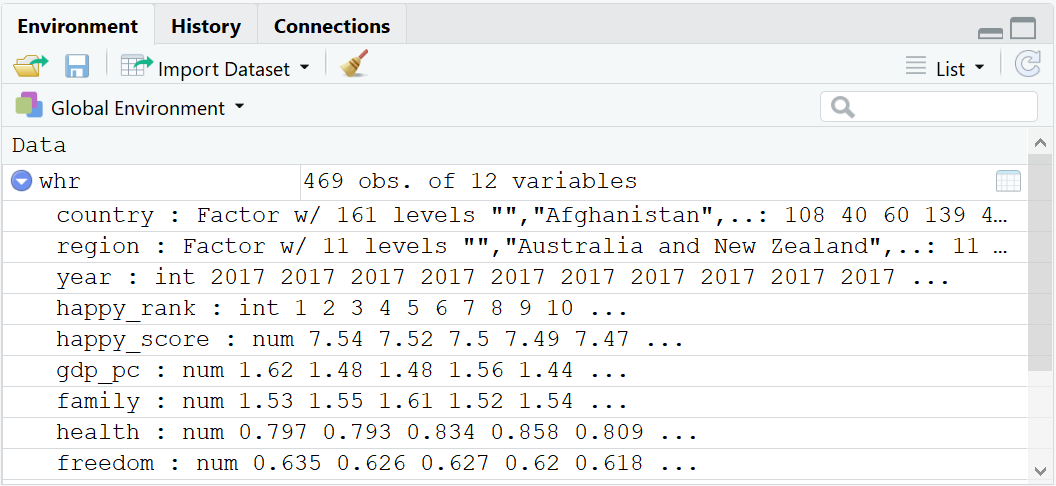
\includegraphics[scale=0.46]{img/enviroment_factors.png}
\end{figure}

\end{frame}

\begin{frame}{Advanced types of data}

\framesubtitle{Factors}

We'll learn how to deal with factors in detail on the next session,
since they are very important for us. For now, here are two important
things to keep in mind when using them:

\begin{block}{Warning:}

Unlike Stata, in R

\begin{enumerate}
\def\labelenumi{\arabic{enumi}.}
\tightlist
\item
  You use the labels to refer to factors
\item
  You cannot choose the underlying values
\end{enumerate}

\end{block}

\end{frame}

\begin{frame}[fragile]{Advanced types of data}

\framesubtitle{Booleans}

Boolean data is the result of logical conditions

\begin{itemize}
\tightlist
\item
  Whenever you're using an \texttt{if} statement in Stata, you're
  implicitly using boolean data.
\item
  The difference is that in R, this can be done in 2 steps.
\end{itemize}

\end{frame}

\begin{frame}[fragile]{Advanced types of data}

\framesubtitle{Booleans}

\begin{block}{Exercise 6:}

Create boolean vector with the condition of annual income below average:

\begin{Shaded}
\begin{Highlighting}[]
\CommentTok{# Create vector}
\NormalTok{bool_vec <-}\StringTok{ }\NormalTok{(whr}\OperatorTok{$}\NormalTok{happy_rank }\OperatorTok{<}
\StringTok{               }\KeywordTok{mean}\NormalTok{(whr}\OperatorTok{$}\NormalTok{happy_rank))}

\CommentTok{# See the 5 first elements of the vector}
\KeywordTok{head}\NormalTok{(bool_vec)}
\end{Highlighting}
\end{Shaded}

\begin{verbatim}
## [1] TRUE TRUE TRUE TRUE TRUE TRUE
\end{verbatim}

\end{block}

\end{frame}

\begin{frame}[fragile]{Advanced types of data}

\framesubtitle{Booleans}

Let's use the boolean vector created to add a dummy variable in the
\texttt{whr} data set for the same condition.

\begin{block}{Exercise 6:}

\begin{enumerate}
\def\labelenumi{\arabic{enumi}.}
\tightlist
\item
  Create a column in \texttt{whr} containing zeros and call it
  \texttt{rank\_low}. You can do this by typing:
\end{enumerate}

\begin{Shaded}
\begin{Highlighting}[]
\NormalTok{whr}\OperatorTok{$}\NormalTok{rank_low <-}\StringTok{ }\DecValTok{0}
\end{Highlighting}
\end{Shaded}

\begin{enumerate}
\def\labelenumi{\arabic{enumi}.}
\setcounter{enumi}{1}
\tightlist
\item
  Use \texttt{bool\_vec} to index the lines of the \texttt{income\_low}
  column and replace all observations that meet the condition with the
  value 1.
\end{enumerate}

\begin{Shaded}
\begin{Highlighting}[]
\NormalTok{whr}\OperatorTok{$}\NormalTok{rank_low[bool_vec] <-}\StringTok{ }\DecValTok{1}
\end{Highlighting}
\end{Shaded}

\end{block}

\end{frame}

\begin{frame}[fragile]{Advanced types of data}

\framesubtitle{Booleans}

\begin{Shaded}
\begin{Highlighting}[]
\CommentTok{# Replace with 1 those obs that meet the condition}
\NormalTok{whr}\OperatorTok{$}\NormalTok{rank_low [bool_vec] <-}\StringTok{ }\DecValTok{1} 
\CommentTok{# is the same as}
\NormalTok{whr}\OperatorTok{$}\NormalTok{rank_low[whr}\OperatorTok{$}\NormalTok{happy_rank }\OperatorTok{<}\StringTok{ }\KeywordTok{mean}\NormalTok{(whr}\OperatorTok{$}\NormalTok{happy_rank)] <-}\StringTok{ }\DecValTok{1} 
\CommentTok{# This in stata would be }
\CommentTok{# replace rank_low = 1 if (...)}


\CommentTok{# We can use the summary function to get descriptives}
\KeywordTok{summary}\NormalTok{(whr}\OperatorTok{$}\NormalTok{rank_low)}
\end{Highlighting}
\end{Shaded}

\begin{verbatim}
##    Min. 1st Qu.  Median    Mean 3rd Qu.    Max. 
##  0.0000  0.0000  0.0000  0.4979  1.0000  1.0000
\end{verbatim}

\end{frame}

\end{document}
